% 01-Introduccion_Presentacion_Tesis.tex
% Diapositivas de la sección Introducción

\section{Introducción}

\begin{frame}
\frametitle{Contexto: COVID-19 y Salud Pública}
\begin{itemize}
    \item La pandemia de COVID-19 ha tenido un impacto sin precedentes:
    \begin{itemize}
        \item En salud y el bienestar de las personas
        \item En sistemas de salud a nivel mundial
    \end{itemize}
\end{itemize}

\begin{itemize}
    \item Alta demanda de atención médica
    \begin{itemize}
        \item Provocó saturación hospitalaria.
        \item Evidenció vulnerabilidad de los trabajadores de la salud.
    \end{itemize}
\end{itemize}
\end{frame}

\begin{frame}
\frametitle{Historia y Desafíos del COVID-19}
\begin{itemize}
    \item COVID-19 surge en 2019 en Wuhan, China, y es declarada pandemia en marzo de 2020.
    \item La ciencia y tecnología se convierten en herramientas clave para enfrentar estos retos.
    \item Urgencia de métodos que agilicen el diagnóstico y tratamiento de enfermedades pulmonares.
\end{itemize}
\end{frame}

\begin{frame}
\frametitle{Diagnóstico por Imágenes y Aprendizaje Automático}
\begin{itemize}
    \item El análisis de imágenes de rayos X y TC es fundamental para el diagnóstico de enfermedades pulmonares.
    \item Modelos de inteligencia artificial ayudan a identificar patologías y visualizar regiones de interés.
    \item Mejoran la precisión y rapidez del diagnóstico, optimizando recursos hospitalarios.
\end{itemize}
\begin{figure}[ht!]
    \centering
    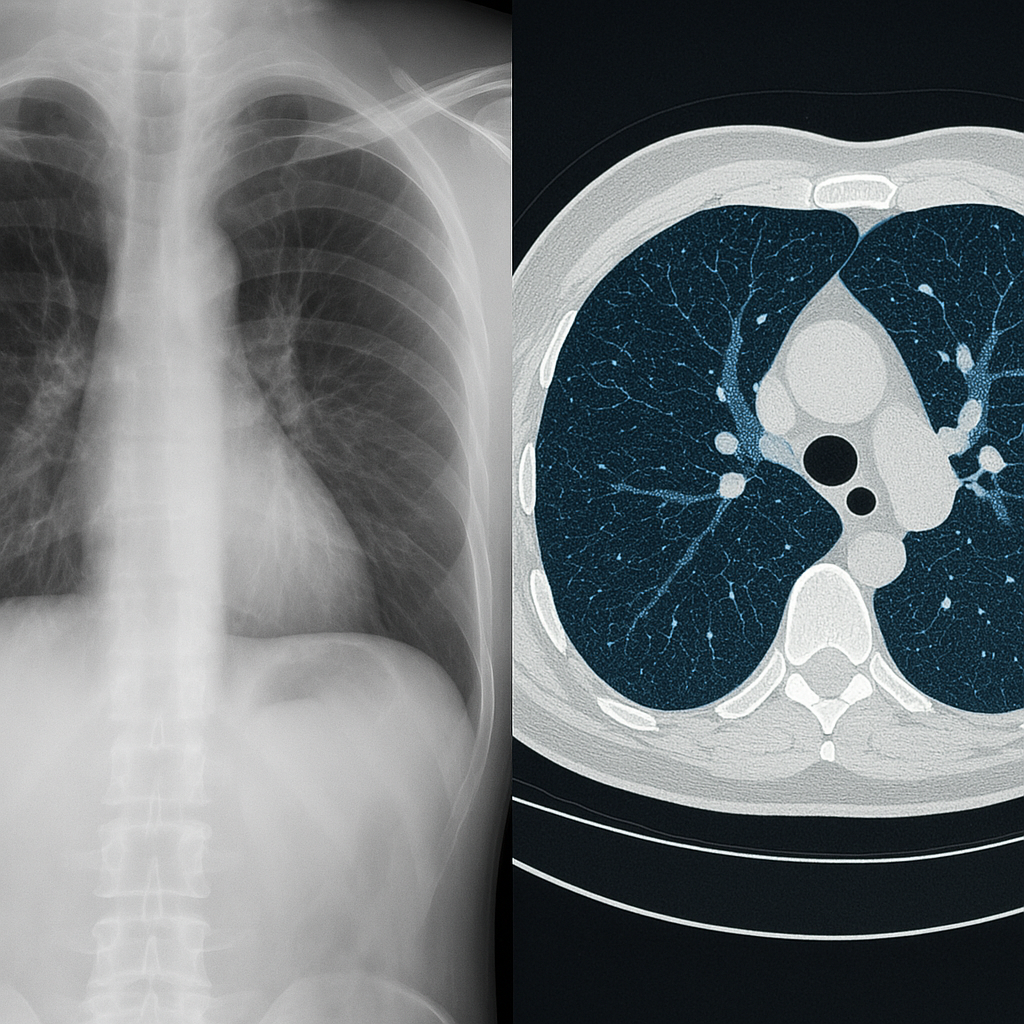
\includegraphics[width=0.2\textwidth]{images/x-ray-tc.png}
    \caption{Ilustración de una imagen de rayos X y un TC.}
\end{figure}
\end{frame}

\begin{frame}
\frametitle{Estado Actual de la Investigación}
\begin{itemize}
    \item A pesar de los avances, los métodos actuales enfrentan limitaciones importantes:
    \begin{itemize}
        \item Sesgos por bases de datos pequeñas o no normalizadas.
        \item Enfoques limitados a enfermedades específicas.
        \item Falta de regulación, validación y explicabilidad de los modelos.
    \end{itemize}
    \item Estas limitaciones dificultan su aplicación en entornos clínicos.
\end{itemize}
\end{frame}
